\documentclass[twoside]{book}

% Packages required by doxygen
\usepackage{fixltx2e}
\usepackage{calc}
\usepackage{doxygen}
\usepackage[export]{adjustbox} % also loads graphicx
\usepackage{graphicx}
\usepackage[utf8]{inputenc}
\usepackage{makeidx}
\usepackage{multicol}
\usepackage{multirow}
\PassOptionsToPackage{warn}{textcomp}
\usepackage{textcomp}
\usepackage[nointegrals]{wasysym}
\usepackage[table]{xcolor}

% Font selection
\usepackage[T1]{fontenc}
\usepackage[scaled=.90]{helvet}
\usepackage{courier}
\usepackage{amssymb}
\usepackage{sectsty}
\renewcommand{\familydefault}{\sfdefault}
\allsectionsfont{%
  \fontseries{bc}\selectfont%
  \color{darkgray}%
}
\renewcommand{\DoxyLabelFont}{%
  \fontseries{bc}\selectfont%
  \color{darkgray}%
}
\newcommand{\+}{\discretionary{\mbox{\scriptsize$\hookleftarrow$}}{}{}}

% Page & text layout
\usepackage{geometry}
\geometry{%
  a4paper,%
  top=2.5cm,%
  bottom=2.5cm,%
  left=2.5cm,%
  right=2.5cm%
}
\tolerance=750
\hfuzz=15pt
\hbadness=750
\setlength{\emergencystretch}{15pt}
\setlength{\parindent}{0cm}
\setlength{\parskip}{3ex plus 2ex minus 2ex}
\makeatletter
\renewcommand{\paragraph}{%
  \@startsection{paragraph}{4}{0ex}{-1.0ex}{1.0ex}{%
    \normalfont\normalsize\bfseries\SS@parafont%
  }%
}
\renewcommand{\subparagraph}{%
  \@startsection{subparagraph}{5}{0ex}{-1.0ex}{1.0ex}{%
    \normalfont\normalsize\bfseries\SS@subparafont%
  }%
}
\makeatother

% Headers & footers
\usepackage{fancyhdr}
\pagestyle{fancyplain}
\fancyhead[LE]{\fancyplain{}{\bfseries\thepage}}
\fancyhead[CE]{\fancyplain{}{}}
\fancyhead[RE]{\fancyplain{}{\bfseries\leftmark}}
\fancyhead[LO]{\fancyplain{}{\bfseries\rightmark}}
\fancyhead[CO]{\fancyplain{}{}}
\fancyhead[RO]{\fancyplain{}{\bfseries\thepage}}
\fancyfoot[LE]{\fancyplain{}{}}
\fancyfoot[CE]{\fancyplain{}{}}
\fancyfoot[RE]{\fancyplain{}{\bfseries\scriptsize Generated by Doxygen }}
\fancyfoot[LO]{\fancyplain{}{\bfseries\scriptsize Generated by Doxygen }}
\fancyfoot[CO]{\fancyplain{}{}}
\fancyfoot[RO]{\fancyplain{}{}}
\renewcommand{\footrulewidth}{0.4pt}
\renewcommand{\chaptermark}[1]{%
  \markboth{#1}{}%
}
\renewcommand{\sectionmark}[1]{%
  \markright{\thesection\ #1}%
}

% Indices & bibliography
\usepackage{natbib}
\usepackage[titles]{tocloft}
\setcounter{tocdepth}{3}
\setcounter{secnumdepth}{5}
\makeindex

% Hyperlinks (required, but should be loaded last)
\usepackage{ifpdf}
\ifpdf
  \usepackage[pdftex,pagebackref=true]{hyperref}
\else
  \usepackage[ps2pdf,pagebackref=true]{hyperref}
\fi
\hypersetup{%
  colorlinks=true,%
  linkcolor=blue,%
  citecolor=blue,%
  unicode%
}

% Custom commands
\newcommand{\clearemptydoublepage}{%
  \newpage{\pagestyle{empty}\cleardoublepage}%
}

\usepackage{caption}
\captionsetup{labelsep=space,justification=centering,font={bf},singlelinecheck=off,skip=4pt,position=top}

%===== C O N T E N T S =====

\begin{document}

% Titlepage & ToC
\hypersetup{pageanchor=false,
             bookmarksnumbered=true,
             pdfencoding=unicode
            }
\pagenumbering{roman}
\begin{titlepage}
\vspace*{7cm}
\begin{center}%
{\Large Dual Degree Project }\\
\vspace*{1cm}
{\large Generated by Doxygen 1.8.11}\\
\end{center}
\end{titlepage}
\clearemptydoublepage
\tableofcontents
\clearemptydoublepage
\pagenumbering{arabic}
\hypersetup{pageanchor=true}

%--- Begin generated contents ---
\chapter{My Personal Index Page}
\label{index}\hypertarget{index}{}\hypertarget{index_intro_sec}{}\section{Introduction}\label{index_intro_sec}
This is the C++ code to solve the high speed fluid flow. Currently, Euler flow is being solved but this code has been designed in moulder way so to solve the viscus flow additional viscus flux class can be added very easily. This code has been written to fulfill the requirement of the Dual Degree Project(\+D\+D\+P).\hypertarget{index_install_sec}{}\section{Installation \& Use}\label{index_install_sec}
To use the solver. Follow these simple steps.
\begin{DoxyItemize}
\item Download form here \+: \href{https://github.com/singh-kuldeep/DDP2}{\tt https\+://github.\+com/singh-\/kuldeep/\+D\+D\+P2} or \href{https://github.com/singh-kuldeep/DDP2}{\tt click here}
\item Go to the folder D\+D\+P2 and compile and run the file \hyperlink{TVD_8cpp}{T\+V\+D.\+cpp} (ex. g++ \hyperlink{TVD_8cpp}{T\+V\+D.\+cpp} \&\& ./a.out)
\item Nozzle has been set up as a default geometry but it can be changed from \char`\"{}run.\+h\char`\"{} file by uncommenting the header file
\item Currently there are two different geometry options are available
\begin{DoxyEnumerate}
\item Curved wall high area ratio diverging nozzle
\item Triangular bump inside straight duct
\end{DoxyEnumerate}
\end{DoxyItemize}\hypertarget{index_brief}{}\section{Brief about the solver}\label{index_brief}

\begin{DoxyItemize}
\item 3D Cartesian (x,y,z)
\item Roe scheme based
\item C++
\item Exact theory can be found \href{https://drive.google.com/open?id=0B9x_nh0D_HhzMnBjc0w5MmJpcnc}{\tt here}
\end{DoxyItemize}\hypertarget{index_input}{}\section{Input to the solver}\label{index_input}

\begin{DoxyItemize}
\item Grid points
\item Boundary condition
\item Some initial condition 
\end{DoxyItemize}\hypertarget{index_output}{}\section{Output files.}\label{index_output}
Here are the list of files which will come as the output of the solver.
\begin{DoxyItemize}
\item Residual\+\_\+\+Nozzle.\+csv \+: This file contains the all the residuals (Mass, Momentum, Energy).
\item grids\+\_\+\+Nozzle\+\_\+2\+D.\+csv \+: This file contains the grid point (x,y) coordinates.
\item 2\+D\+\_\+parameters\+\_\+\+B.\+csv \+: This file contains all the conserved parameters at the 2D plane. 
\end{DoxyItemize}\hypertarget{index_plot}{}\section{Results \& Plots}\label{index_plot}
Same older contains the M\+A\+T\+L\+AB script \char`\"{}plot\+\_\+data.\+m\char`\"{}. Once the simulation has started and the output files are generated, one can simply run the M\+A\+T\+A\+LB script and can see the plots which are listed below.
\begin{DoxyItemize}
\item Density Residual
\item X Momentum Residual
\item Y Momentum Residual
\item Z Momentum Residual
\item Energy Residual
\item Mach Number
\item Density
\item Velocity
\item Temperature
\item Pressure
\item Geometry 2D cross section 
\end{DoxyItemize}
\chapter{Bug List}
\label{bug}
\hypertarget{bug}{}

\begin{DoxyRefList}
\item[\label{bug__bug000001}%
\hypertarget{bug__bug000001}{}%
Member \hyperlink{classdiffusionfluxinterface_a30feb61f31b2c40063fc4ca7ca16258e}{diffusionfluxinterface\+:\+:diffusionfluxinterface} (vector$<$ double $>$ \&Conserved\+Variable\+Left\+Minus, vector$<$ double $>$ \&Conserved\+Variable\+Left, vector$<$ double $>$ \&Conserved\+Variable\+Right, vector$<$ double $>$ \&Conserved\+Variable\+Right\+Plus, vector$<$ double $>$ \&Face\+Area\+Vector\+Left, vector$<$ double $>$ \&Face\+Area\+Vector\+Right, vector$<$ double $>$ \&Face\+Area\+Vector\+Right\+Plus, double Cell\+Volume\+Left\+Mins, double Cell\+Volume\+Left, double Cell\+Volume\+Right, double Cell\+Volume\+Right\+Plus, double DeltaT)]Here syntax needs to be changed for gvactor\mbox{[}i\mbox{]} calculation 

Here I have doubt about \char`\"{}not equal to sign\char`\"{} because it can\textquotesingle{}t be exactly equal to 0.\+00000 so most of the time we end up choosing theta i = 0.\+0  
\item[\label{bug__bug000003}%
\hypertarget{bug__bug000003}{}%
File \hyperlink{dt_8h}{dt.h} ]Currently not using this, because \hyperlink{grid__nozzle_8h_a6cdf5cf168063009e847db46d6624c1b}{grid()} is not calculating ds value. So recheck this function as well after fixing the \hyperlink{grid__nozzle_8h_a6cdf5cf168063009e847db46d6624c1b}{grid()} function.  
\item[\label{bug__bug000004}%
\hypertarget{bug__bug000004}{}%
File \hyperlink{eulerflux_8h}{eulerflux.h} ]Not all memory is freed when deleting an object of this class.  
\item[\label{bug__bug000005}%
\hypertarget{bug__bug000005}{}%
Member \hyperlink{run_8h_ac7609273a01eb63ff8a25ddf1aafeff7}{grid} (vector$<$ vector$<$ vector$<$ vector$<$ double $>$ $>$ $>$ $>$ \&i\+Face\+Area\+Vector, vector$<$ vector$<$ vector$<$ vector$<$ double $>$ $>$ $>$ $>$ \&j\+Face\+Area\+Vector, vector$<$ vector$<$ vector$<$ vector$<$ double $>$ $>$ $>$ $>$ \&k\+Face\+Area\+Vector, vector$<$ vector$<$ vector$<$ double $>$ $>$ $>$ \&Cell\+Volume, vector$<$ vector$<$ vector$<$ double $>$ $>$ $>$ \&delta\+\_\+s, int \&Ni, int \&Nj, int \&Nk)]Yet to calculate the ds value properly  
\item[\label{bug__bug000005}%
\hypertarget{bug__bug000005}{}%
Member \hyperlink{run_8h_ac7609273a01eb63ff8a25ddf1aafeff7}{grid} (vector$<$ vector$<$ vector$<$ vector$<$ double $>$ $>$ $>$ $>$ \&i\+Face\+Area\+Vector, vector$<$ vector$<$ vector$<$ vector$<$ double $>$ $>$ $>$ $>$ \&j\+Face\+Area\+Vector, vector$<$ vector$<$ vector$<$ vector$<$ double $>$ $>$ $>$ $>$ \&k\+Face\+Area\+Vector, vector$<$ vector$<$ vector$<$ double $>$ $>$ $>$ \&Cell\+Volume, vector$<$ vector$<$ vector$<$ double $>$ $>$ $>$ \&delta\+\_\+s, int \&Ni, int \&Nj, int \&Nk)]Yet to calculate the ds value properly  
\item[\label{bug__bug000006}%
\hypertarget{bug__bug000006}{}%
Member \hyperlink{run_8h_a13a43e6d814de94978c515cb084873b1}{run} ()]Every time simulation starts from first iteration. So, to save the simulation it is good to start from the last solution as the initial condition 

Local time step needs to be used to reduce the simulation time 
\end{DoxyRefList}
\chapter{Class Index}
\section{Class List}
Here are the classes, structs, unions and interfaces with brief descriptions\+:\begin{DoxyCompactList}
\item\contentsline{section}{\hyperlink{classdiffusionfluxAUSM}{diffusionflux\+A\+U\+SM} }{\pageref{classdiffusionfluxAUSM}}{}
\item\contentsline{section}{\hyperlink{classdiffusionfluxinterface}{diffusionfluxinterface} }{\pageref{classdiffusionfluxinterface}}{}
\item\contentsline{section}{\hyperlink{classeulerflux}{eulerflux} }{\pageref{classeulerflux}}{}
\item\contentsline{section}{\hyperlink{classeulerfluxAUSM}{eulerflux\+A\+U\+SM} }{\pageref{classeulerfluxAUSM}}{}
\item\contentsline{section}{\hyperlink{classinterface}{interface} }{\pageref{classinterface}}{}
\item\contentsline{section}{\hyperlink{classnetfluxAUSM}{netflux\+A\+U\+SM} }{\pageref{classnetfluxAUSM}}{}
\item\contentsline{section}{\hyperlink{structnetfluxBase}{netflux\+Base} }{\pageref{structnetfluxBase}}{}
\item\contentsline{section}{\hyperlink{classnetfluxRoe}{netflux\+Roe} }{\pageref{classnetfluxRoe}}{}
\end{DoxyCompactList}

\chapter{File Index}
\section{File List}
Here is a list of all documented files with brief descriptions\+:\begin{DoxyCompactList}
\item\contentsline{section}{\hyperlink{BC_8h}{B\+C.\+h} \\*This header file implements all three boundary conditions }{\pageref{BC_8h}}{}
\item\contentsline{section}{\hyperlink{diffusionfluxinterface_8h}{diffusionfluxinterface.\+h} \\*This class calculates the numerical diffusion flux }{\pageref{diffusionfluxinterface_8h}}{}
\item\contentsline{section}{\hyperlink{dt_8h}{dt.\+h} \\*This header file conditions the function Time\+Step() which calculate the local time step for each cell at every iteration }{\pageref{dt_8h}}{}
\item\contentsline{section}{\hyperlink{eulerflux_8h}{eulerflux.\+h} \\*This class calculates the euler flux vectors(\+Ee,\+Fe,\+Ge) at the interface }{\pageref{eulerflux_8h}}{}
\item\contentsline{section}{{\bfseries grid\+\_\+diverging\+\_\+duct.\+h} }{\pageref{grid__diverging__duct_8h}}{}
\item\contentsline{section}{\hyperlink{grid__nozzle_8h}{grid\+\_\+nozzle.\+h} \\*This header file functions find the grid points, cell area vectors and the cell volumes }{\pageref{grid__nozzle_8h}}{}
\item\contentsline{section}{\hyperlink{interface_8h}{interface.\+h} \\*This class calculates the interface parameters using Reo scheme flux }{\pageref{interface_8h}}{}
\item\contentsline{section}{\hyperlink{netfluxinterface_8h}{netfluxinterface.\+h} \\*Calculates the net flux vector(numerical diffusion and euler flux) at the interface }{\pageref{netfluxinterface_8h}}{}
\item\contentsline{section}{\hyperlink{run_8h}{run.\+h} \\*This header file contains the \hyperlink{run_8h_a13a43e6d814de94978c515cb084873b1}{run()} function which runs the solver }{\pageref{run_8h}}{}
\end{DoxyCompactList}

\chapter{Class Documentation}
\hypertarget{classdiffusionfluxAUSM}{}\section{diffusionflux\+A\+U\+SM Class Reference}
\label{classdiffusionfluxAUSM}\index{diffusionflux\+A\+U\+SM@{diffusionflux\+A\+U\+SM}}
\subsection*{Public Member Functions}
\begin{DoxyCompactItemize}
\item 
{\bfseries diffusionflux\+A\+U\+SM} (vector$<$ double $>$ \&Conserved\+Variable, vector$<$ double $>$ \&Area\+Vector)\hypertarget{classdiffusionfluxAUSM_a8b268fcf5178b72c4fa71b9655c0464c}{}\label{classdiffusionfluxAUSM_a8b268fcf5178b72c4fa71b9655c0464c}

\end{DoxyCompactItemize}
\subsection*{Public Attributes}
\begin{DoxyCompactItemize}
\item 
double {\bfseries Flux} \mbox{[}5\mbox{]}\hypertarget{classdiffusionfluxAUSM_af39fcc75248a5e8c8820b1e8609857bc}{}\label{classdiffusionfluxAUSM_af39fcc75248a5e8c8820b1e8609857bc}

\end{DoxyCompactItemize}


The documentation for this class was generated from the following file\+:\begin{DoxyCompactItemize}
\item 
diffusionflux\+A\+U\+S\+M.\+h\end{DoxyCompactItemize}

\hypertarget{classdiffusionfluxinterface}{}\section{diffusionfluxinterface Class Reference}
\label{classdiffusionfluxinterface}\index{diffusionfluxinterface@{diffusionfluxinterface}}
\subsection*{Public Member Functions}
\begin{DoxyCompactItemize}
\item 
\hyperlink{classdiffusionfluxinterface_a30feb61f31b2c40063fc4ca7ca16258e}{diffusionfluxinterface} (vector$<$ double $>$ \&Conserved\+Variable\+Left\+Minus, vector$<$ double $>$ \&Conserved\+Variable\+Left, vector$<$ double $>$ \&Conserved\+Variable\+Right, vector$<$ double $>$ \&Conserved\+Variable\+Right\+Plus, vector$<$ double $>$ \&Face\+Area\+Vector\+Left, vector$<$ double $>$ \&Face\+Area\+Vector\+Right, vector$<$ double $>$ \&Face\+Area\+Vector\+Right\+Plus, double Cell\+Volume\+Left\+Mins, double Cell\+Volume\+Left, double Cell\+Volume\+Right, double Cell\+Volume\+Right\+Plus, double DeltaT)
\end{DoxyCompactItemize}
\subsection*{Public Attributes}
\begin{DoxyCompactItemize}
\item 
double {\bfseries Diffusion\+Flux\+Vector} \mbox{[}5\mbox{]}\hypertarget{classdiffusionfluxinterface_a2e1da15c8bd0876ddb087c5cab930a28}{}\label{classdiffusionfluxinterface_a2e1da15c8bd0876ddb087c5cab930a28}

\end{DoxyCompactItemize}


\subsection{Constructor \& Destructor Documentation}
\index{diffusionfluxinterface@{diffusionfluxinterface}!diffusionfluxinterface@{diffusionfluxinterface}}
\index{diffusionfluxinterface@{diffusionfluxinterface}!diffusionfluxinterface@{diffusionfluxinterface}}
\subsubsection[{\texorpdfstring{diffusionfluxinterface(vector$<$ double $>$ \&\+Conserved\+Variable\+Left\+Minus, vector$<$ double $>$ \&\+Conserved\+Variable\+Left, vector$<$ double $>$ \&\+Conserved\+Variable\+Right, vector$<$ double $>$ \&\+Conserved\+Variable\+Right\+Plus, vector$<$ double $>$ \&\+Face\+Area\+Vector\+Left, vector$<$ double $>$ \&\+Face\+Area\+Vector\+Right, vector$<$ double $>$ \&\+Face\+Area\+Vector\+Right\+Plus, double Cell\+Volume\+Left\+Mins, double Cell\+Volume\+Left, double Cell\+Volume\+Right, double Cell\+Volume\+Right\+Plus, double Delta\+T)}{diffusionfluxinterface(vector< double > &ConservedVariableLeftMinus, vector< double > &ConservedVariableLeft, vector< double > &ConservedVariableRight, vector< double > &ConservedVariableRightPlus, vector< double > &FaceAreaVectorLeft, vector< double > &FaceAreaVectorRight, vector< double > &FaceAreaVectorRightPlus, double CellVolumeLeftMins, double CellVolumeLeft, double CellVolumeRight, double CellVolumeRightPlus, double DeltaT)}}]{\setlength{\rightskip}{0pt plus 5cm}diffusionfluxinterface\+::diffusionfluxinterface (
\begin{DoxyParamCaption}
\item[{vector$<$ double $>$ \&}]{Conserved\+Variable\+Left\+Minus, }
\item[{vector$<$ double $>$ \&}]{Conserved\+Variable\+Left, }
\item[{vector$<$ double $>$ \&}]{Conserved\+Variable\+Right, }
\item[{vector$<$ double $>$ \&}]{Conserved\+Variable\+Right\+Plus, }
\item[{vector$<$ double $>$ \&}]{Face\+Area\+Vector\+Left, }
\item[{vector$<$ double $>$ \&}]{Face\+Area\+Vector\+Right, }
\item[{vector$<$ double $>$ \&}]{Face\+Area\+Vector\+Right\+Plus, }
\item[{double}]{Cell\+Volume\+Left\+Mins, }
\item[{double}]{Cell\+Volume\+Left, }
\item[{double}]{Cell\+Volume\+Right, }
\item[{double}]{Cell\+Volume\+Right\+Plus, }
\item[{double}]{DeltaT}
\end{DoxyParamCaption}
)\hspace{0.3cm}{\ttfamily [inline]}}\hypertarget{classdiffusionfluxinterface_a30feb61f31b2c40063fc4ca7ca16258e}{}\label{classdiffusionfluxinterface_a30feb61f31b2c40063fc4ca7ca16258e}
\begin{DoxyRefDesc}{Bug}
\item[\hyperlink{bug__bug000002}{Bug}]Here syntax needs to be changed for gvactor\mbox{[}i\mbox{]} calculation \end{DoxyRefDesc}


\begin{DoxyRefDesc}{Bug}
\item[\hyperlink{bug__bug000003}{Bug}]Here I have doubt about \char`\"{}not equal to sign\char`\"{} because it can\textquotesingle{}t be exactly equal to 0.\+00000 so most of the time we end up choosing theta i = 0.\+0 \end{DoxyRefDesc}


The documentation for this class was generated from the following file\+:\begin{DoxyCompactItemize}
\item 
\hyperlink{diffusionfluxinterface_8h}{diffusionfluxinterface.\+h}\end{DoxyCompactItemize}

\hypertarget{classeulerflux}{}\section{eulerflux Class Reference}
\label{classeulerflux}\index{eulerflux@{eulerflux}}
\subsection*{Public Member Functions}
\begin{DoxyCompactItemize}
\item 
\hyperlink{classeulerflux_a184f13dbf2a62b11c443688049c1f4db}{eulerflux} (vector$<$ double $>$ \&Conserved\+Variable)
\end{DoxyCompactItemize}
\subsection*{Public Attributes}
\begin{DoxyCompactItemize}
\item 
double {\bfseries Euler\+FluxX} \mbox{[}5\mbox{]}\hypertarget{classeulerflux_a0282624fae997ac54441271130497185}{}\label{classeulerflux_a0282624fae997ac54441271130497185}

\item 
double {\bfseries Euler\+FluxY} \mbox{[}5\mbox{]}\hypertarget{classeulerflux_afdebc952e09629e73d7dcdda3e9e60ce}{}\label{classeulerflux_afdebc952e09629e73d7dcdda3e9e60ce}

\item 
double {\bfseries Euler\+FluxZ} \mbox{[}5\mbox{]}\hypertarget{classeulerflux_aaf2a28c94cb1cad57800342f8496c4b2}{}\label{classeulerflux_aaf2a28c94cb1cad57800342f8496c4b2}

\end{DoxyCompactItemize}


\subsection{Constructor \& Destructor Documentation}
\index{eulerflux@{eulerflux}!eulerflux@{eulerflux}}
\index{eulerflux@{eulerflux}!eulerflux@{eulerflux}}
\subsubsection[{\texorpdfstring{eulerflux(vector$<$ double $>$ \&\+Conserved\+Variable)}{eulerflux(vector< double > &ConservedVariable)}}]{\setlength{\rightskip}{0pt plus 5cm}eulerflux\+::eulerflux (
\begin{DoxyParamCaption}
\item[{vector$<$ double $>$ \&}]{Conserved\+Variable}
\end{DoxyParamCaption}
)\hspace{0.3cm}{\ttfamily [inline]}}\hypertarget{classeulerflux_a184f13dbf2a62b11c443688049c1f4db}{}\label{classeulerflux_a184f13dbf2a62b11c443688049c1f4db}

\begin{DoxyParams}[1]{Parameters}
 & {\em Euler\+FluxX} & x direction euler flux vector (Ee) at interface \\
\hline
 & {\em Euler\+FluxY} & y direction euler flux vector (Fe) at interface \\
\hline
 & {\em Euler\+FluxZ} & z direction euler flux vector (Ge) at interface \\
\hline
\mbox{\tt in}  & {\em Conserved\+Variable} & Conserved variable vector (\mbox{[}Density , x-\/momentum, y-\/momentum, z-\/momentum, Energy\mbox{]}) \\
\hline
 & {\em Pressure} & Satic pressure (p) \\
\hline
\end{DoxyParams}


The documentation for this class was generated from the following file\+:\begin{DoxyCompactItemize}
\item 
\hyperlink{eulerflux_8h}{eulerflux.\+h}\end{DoxyCompactItemize}

\hypertarget{classeulerfluxAUSM}{}\section{eulerflux\+A\+U\+SM Class Reference}
\label{classeulerfluxAUSM}\index{eulerflux\+A\+U\+SM@{eulerflux\+A\+U\+SM}}


This class calculates the Euler flux vectors(\+Ee,\+Fe,\+Ge) at the interface for the A\+U\+SM scheme.  




{\ttfamily \#include $<$Convective\+Flux\+A\+U\+S\+M.\+h$>$}

\subsection*{Public Member Functions}
\begin{DoxyCompactItemize}
\item 
\hyperlink{classeulerfluxAUSM_a313596688131132478810bf14c0701ae}{eulerflux\+A\+U\+SM} (vector$<$ double $>$ Conserved\+Variable, vector$<$ double $>$ Area\+Vector, string gamma, double Specific\+Heat\+Ratio)
\end{DoxyCompactItemize}
\subsection*{Public Attributes}
\begin{DoxyCompactItemize}
\item 
double \hyperlink{classeulerfluxAUSM_a46908ae326123ac416f7ae023c280060}{Flux} \mbox{[}5\mbox{]}
\item 
double \hyperlink{classeulerfluxAUSM_a9565c076f0be6c66124056ed3fff66b7}{Mach\+Plus}
\item 
double \hyperlink{classeulerfluxAUSM_a8a114564c03cd55a32e0255f9bddbd20}{Mach\+Minus}
\item 
double \hyperlink{classeulerfluxAUSM_abfd3213993dd4b53b12c3f5ecd7046e5}{Pressure\+Plus}
\item 
double \hyperlink{classeulerfluxAUSM_a509830d732c5117ce212397b07e60720}{Pressure\+Minus}
\item 
double \hyperlink{classeulerfluxAUSM_a7c9560ef18e086f6d3cc376c151ad2ff}{Mach}
\end{DoxyCompactItemize}


\subsection{Detailed Description}
This class calculates the Euler flux vectors(\+Ee,\+Fe,\+Ge) at the interface for the A\+U\+SM scheme. 

\begin{DoxyDate}{Date}
18-\/\+May-\/2017 
\end{DoxyDate}


\subsection{Constructor \& Destructor Documentation}
\index{eulerflux\+A\+U\+SM@{eulerflux\+A\+U\+SM}!eulerflux\+A\+U\+SM@{eulerflux\+A\+U\+SM}}
\index{eulerflux\+A\+U\+SM@{eulerflux\+A\+U\+SM}!eulerflux\+A\+U\+SM@{eulerflux\+A\+U\+SM}}
\subsubsection[{\texorpdfstring{eulerflux\+A\+U\+S\+M(vector$<$ double $>$ Conserved\+Variable, vector$<$ double $>$ Area\+Vector, string gamma, double Specific\+Heat\+Ratio)}{eulerfluxAUSM(vector< double > ConservedVariable, vector< double > AreaVector, string gamma, double SpecificHeatRatio)}}]{\setlength{\rightskip}{0pt plus 5cm}eulerflux\+A\+U\+S\+M\+::eulerflux\+A\+U\+SM (
\begin{DoxyParamCaption}
\item[{vector$<$ double $>$}]{Conserved\+Variable, }
\item[{vector$<$ double $>$}]{Area\+Vector, }
\item[{string}]{gamma, }
\item[{double}]{Specific\+Heat\+Ratio}
\end{DoxyParamCaption}
)\hspace{0.3cm}{\ttfamily [inline]}}\hypertarget{classeulerfluxAUSM_a313596688131132478810bf14c0701ae}{}\label{classeulerfluxAUSM_a313596688131132478810bf14c0701ae}
A constructor to calculate the convective flux and initiates the parameter which are required in the flux calculation. 
\begin{DoxyParams}{Parameters}
{\em Conserved\+Variable} & All the conserved variable in the cell \\
\hline
{\em Area\+Vector} & Face area vector \\
\hline
{\em gamma} & String tells whether to consider specific heat ratio is constant or varying with temperature \\
\hline
{\em Specific\+Heat\+Ratio} & Specific heat ratio in case of constant gamma \\
\hline
\end{DoxyParams}

\begin{DoxyParams}{Parameters}
{\em Area\+Vector\+Normal} & Interface unit area vector\\
\hline
{\em Area\+Vector\+Magnitude} & Magnitude of area vector\\
\hline
{\em Velocity\+Normal} & Magnitude of velocity vector normal to the interface, or {\bfseries contravarient velocity }\\
\hline
\end{DoxyParams}


\subsection{Member Data Documentation}
\index{eulerflux\+A\+U\+SM@{eulerflux\+A\+U\+SM}!Flux@{Flux}}
\index{Flux@{Flux}!eulerflux\+A\+U\+SM@{eulerflux\+A\+U\+SM}}
\subsubsection[{\texorpdfstring{Flux}{Flux}}]{\setlength{\rightskip}{0pt plus 5cm}double eulerflux\+A\+U\+S\+M\+::\+Flux\mbox{[}5\mbox{]}}\hypertarget{classeulerfluxAUSM_a46908ae326123ac416f7ae023c280060}{}\label{classeulerfluxAUSM_a46908ae326123ac416f7ae023c280060}

\begin{DoxyParams}{Parameters}
{\em Flux} & Convective flux vector in the cell \\
\hline
\end{DoxyParams}
\index{eulerflux\+A\+U\+SM@{eulerflux\+A\+U\+SM}!Mach@{Mach}}
\index{Mach@{Mach}!eulerflux\+A\+U\+SM@{eulerflux\+A\+U\+SM}}
\subsubsection[{\texorpdfstring{Mach}{Mach}}]{\setlength{\rightskip}{0pt plus 5cm}double eulerflux\+A\+U\+S\+M\+::\+Mach}\hypertarget{classeulerfluxAUSM_a7c9560ef18e086f6d3cc376c151ad2ff}{}\label{classeulerfluxAUSM_a7c9560ef18e086f6d3cc376c151ad2ff}

\begin{DoxyParams}{Parameters}
{\em Mach} & Mach number at the cell \\
\hline
\end{DoxyParams}
\index{eulerflux\+A\+U\+SM@{eulerflux\+A\+U\+SM}!Mach\+Minus@{Mach\+Minus}}
\index{Mach\+Minus@{Mach\+Minus}!eulerflux\+A\+U\+SM@{eulerflux\+A\+U\+SM}}
\subsubsection[{\texorpdfstring{Mach\+Minus}{MachMinus}}]{\setlength{\rightskip}{0pt plus 5cm}double eulerflux\+A\+U\+S\+M\+::\+Mach\+Minus}\hypertarget{classeulerfluxAUSM_a8a114564c03cd55a32e0255f9bddbd20}{}\label{classeulerfluxAUSM_a8a114564c03cd55a32e0255f9bddbd20}

\begin{DoxyParams}{Parameters}
{\em Mach\+Minus} & Mach\+Minus needed in A\+U\+SM scheme, at a the cell \\
\hline
\end{DoxyParams}
\index{eulerflux\+A\+U\+SM@{eulerflux\+A\+U\+SM}!Mach\+Plus@{Mach\+Plus}}
\index{Mach\+Plus@{Mach\+Plus}!eulerflux\+A\+U\+SM@{eulerflux\+A\+U\+SM}}
\subsubsection[{\texorpdfstring{Mach\+Plus}{MachPlus}}]{\setlength{\rightskip}{0pt plus 5cm}double eulerflux\+A\+U\+S\+M\+::\+Mach\+Plus}\hypertarget{classeulerfluxAUSM_a9565c076f0be6c66124056ed3fff66b7}{}\label{classeulerfluxAUSM_a9565c076f0be6c66124056ed3fff66b7}

\begin{DoxyParams}{Parameters}
{\em Mach\+Plus} & Mach\+Plus needed in A\+U\+SM scheme, at a the cell \\
\hline
\end{DoxyParams}
\index{eulerflux\+A\+U\+SM@{eulerflux\+A\+U\+SM}!Pressure\+Minus@{Pressure\+Minus}}
\index{Pressure\+Minus@{Pressure\+Minus}!eulerflux\+A\+U\+SM@{eulerflux\+A\+U\+SM}}
\subsubsection[{\texorpdfstring{Pressure\+Minus}{PressureMinus}}]{\setlength{\rightskip}{0pt plus 5cm}double eulerflux\+A\+U\+S\+M\+::\+Pressure\+Minus}\hypertarget{classeulerfluxAUSM_a509830d732c5117ce212397b07e60720}{}\label{classeulerfluxAUSM_a509830d732c5117ce212397b07e60720}

\begin{DoxyParams}{Parameters}
{\em Pressure\+Minus} & Pressure\+Minus needed in A\+U\+SM scheme, at a the cell \\
\hline
\end{DoxyParams}
\index{eulerflux\+A\+U\+SM@{eulerflux\+A\+U\+SM}!Pressure\+Plus@{Pressure\+Plus}}
\index{Pressure\+Plus@{Pressure\+Plus}!eulerflux\+A\+U\+SM@{eulerflux\+A\+U\+SM}}
\subsubsection[{\texorpdfstring{Pressure\+Plus}{PressurePlus}}]{\setlength{\rightskip}{0pt plus 5cm}double eulerflux\+A\+U\+S\+M\+::\+Pressure\+Plus}\hypertarget{classeulerfluxAUSM_abfd3213993dd4b53b12c3f5ecd7046e5}{}\label{classeulerfluxAUSM_abfd3213993dd4b53b12c3f5ecd7046e5}

\begin{DoxyParams}{Parameters}
{\em Pressure\+Plus} & Pressure\+Plus needed in A\+U\+SM scheme, at a the cell \\
\hline
\end{DoxyParams}


The documentation for this class was generated from the following file\+:\begin{DoxyCompactItemize}
\item 
\hyperlink{ConvectiveFluxAUSM_8h}{Convective\+Flux\+A\+U\+S\+M.\+h}\end{DoxyCompactItemize}

\hypertarget{classinterface}{}\section{interface Class Reference}
\label{classinterface}\index{interface@{interface}}
\subsection*{Public Member Functions}
\begin{DoxyCompactItemize}
\item 
{\bfseries interface} (vector$<$ double $>$ \&Conserved\+Variable\+Left, vector$<$ double $>$ \&Conserved\+Variable\+Right, vector$<$ double $>$ \&Face\+Area\+Vector\+Interface, double Cell\+Volume\+Left, double Cell\+Volume\+Right, double DeltaT)\hypertarget{classinterface_a7abecc6e69fdb7b0dc3a4ad0abbe4f93}{}\label{classinterface_a7abecc6e69fdb7b0dc3a4ad0abbe4f93}

\end{DoxyCompactItemize}
\subsection*{Public Attributes}
\begin{DoxyCompactItemize}
\item 
double {\bfseries Density\+Interface}\hypertarget{classinterface_a5a0a592bdfe7f5987c2c4f4424fbccd9}{}\label{classinterface_a5a0a592bdfe7f5987c2c4f4424fbccd9}

\item 
double {\bfseries Velocity\+X\+Interface}\hypertarget{classinterface_afae6ebb7814474f2264759a14521f448}{}\label{classinterface_afae6ebb7814474f2264759a14521f448}

\item 
double {\bfseries Velocity\+Y\+Interface}\hypertarget{classinterface_a0f42e6e3fd259e9fc191a255a6650ef6}{}\label{classinterface_a0f42e6e3fd259e9fc191a255a6650ef6}

\item 
double {\bfseries Velocity\+Z\+Interface}\hypertarget{classinterface_a1f1cc4570519d23fc38414472d7721f9}{}\label{classinterface_a1f1cc4570519d23fc38414472d7721f9}

\item 
double {\bfseries Enthalpy\+Interface}\hypertarget{classinterface_af2f6d43336396abc20bd88521e489a71}{}\label{classinterface_af2f6d43336396abc20bd88521e489a71}

\item 
double {\bfseries Vector\+Jump\+Interface} \mbox{[}5\mbox{]}\hypertarget{classinterface_aa99760e0d73f30c6f1541414efc76f87}{}\label{classinterface_aa99760e0d73f30c6f1541414efc76f87}

\item 
double {\bfseries Eigen\+Value} \mbox{[}5\mbox{]}\hypertarget{classinterface_a6e63abc816f019315477dc514963c505}{}\label{classinterface_a6e63abc816f019315477dc514963c505}

\item 
double {\bfseries Eigen\+Vector\+Matrix} \mbox{[}5\mbox{]}\mbox{[}5\mbox{]}\hypertarget{classinterface_a5889dedb2a24917fa46bd4c6515a33c7}{}\label{classinterface_a5889dedb2a24917fa46bd4c6515a33c7}

\item 
double {\bfseries Eigen\+Vector\+Matrix\+Inverse} \mbox{[}5\mbox{]}\mbox{[}5\mbox{]}\hypertarget{classinterface_ae67dd839deeeacfb620b114c560ea0a5}{}\label{classinterface_ae67dd839deeeacfb620b114c560ea0a5}

\item 
double {\bfseries Alpha\+Vector\+Interface} \mbox{[}5\mbox{]}\hypertarget{classinterface_aa3f54ad5bd8d3081383f2190090b4109}{}\label{classinterface_aa3f54ad5bd8d3081383f2190090b4109}

\item 
double {\bfseries Mu\+Vector\+Interface} \mbox{[}5\mbox{]}\hypertarget{classinterface_aa740f1171fcddcb604c237cabbcebc1a}{}\label{classinterface_aa740f1171fcddcb604c237cabbcebc1a}

\item 
double {\bfseries Z\+Vector\+Interface} \mbox{[}5\mbox{]}\hypertarget{classinterface_a32902e62056c2479ade3f78167f1522f}{}\label{classinterface_a32902e62056c2479ade3f78167f1522f}

\item 
double {\bfseries Pshi\+Vector\+Interface} \mbox{[}5\mbox{]}\hypertarget{classinterface_a37044e7a6a8820ea4bcbcaf969628238}{}\label{classinterface_a37044e7a6a8820ea4bcbcaf969628238}

\item 
double {\bfseries G\+Vector\+Interface} \mbox{[}5\mbox{]}\hypertarget{classinterface_ab25dbd2f7aaa6921fd5edb973af98ed4}{}\label{classinterface_ab25dbd2f7aaa6921fd5edb973af98ed4}

\end{DoxyCompactItemize}


The documentation for this class was generated from the following file\+:\begin{DoxyCompactItemize}
\item 
\hyperlink{interface_8h}{interface.\+h}\end{DoxyCompactItemize}

\hypertarget{classnetfluxAUSM}{}\section{netflux\+A\+U\+SM Class Reference}
\label{classnetfluxAUSM}\index{netflux\+A\+U\+SM@{netflux\+A\+U\+SM}}


Calculates the net A\+U\+SM flux at the interface.  




{\ttfamily \#include $<$Net\+Flux\+A\+U\+S\+M.\+h$>$}

\subsection*{Public Member Functions}
\begin{DoxyCompactItemize}
\item 
\hyperlink{classnetfluxAUSM_a68c53463497f0c6b3ba8cfc9af17b5cd}{netflux\+A\+U\+SM} (vector$<$ double $>$ Left\+Conserved\+Variable, vector$<$ double $>$ Right\+Conserved\+Variable, vector$<$ double $>$ Area\+Vector, string gamma, double Specific\+Heat\+Ratio)
\end{DoxyCompactItemize}
\subsection*{Public Attributes}
\begin{DoxyCompactItemize}
\item 
double \hyperlink{classnetfluxAUSM_a8fb78535709581ad1f781aff25e61ff9}{Net\+Flux} \mbox{[}5\mbox{]}
\end{DoxyCompactItemize}


\subsection{Detailed Description}
Calculates the net A\+U\+SM flux at the interface. 

\subsection{Constructor \& Destructor Documentation}
\index{netflux\+A\+U\+SM@{netflux\+A\+U\+SM}!netflux\+A\+U\+SM@{netflux\+A\+U\+SM}}
\index{netflux\+A\+U\+SM@{netflux\+A\+U\+SM}!netflux\+A\+U\+SM@{netflux\+A\+U\+SM}}
\subsubsection[{\texorpdfstring{netflux\+A\+U\+S\+M(vector$<$ double $>$ Left\+Conserved\+Variable, vector$<$ double $>$ Right\+Conserved\+Variable, vector$<$ double $>$ Area\+Vector, string gamma, double Specific\+Heat\+Ratio)}{netfluxAUSM(vector< double > LeftConservedVariable, vector< double > RightConservedVariable, vector< double > AreaVector, string gamma, double SpecificHeatRatio)}}]{\setlength{\rightskip}{0pt plus 5cm}netflux\+A\+U\+S\+M\+::netflux\+A\+U\+SM (
\begin{DoxyParamCaption}
\item[{vector$<$ double $>$}]{Left\+Conserved\+Variable, }
\item[{vector$<$ double $>$}]{Right\+Conserved\+Variable, }
\item[{vector$<$ double $>$}]{Area\+Vector, }
\item[{string}]{gamma, }
\item[{double}]{Specific\+Heat\+Ratio}
\end{DoxyParamCaption}
)\hspace{0.3cm}{\ttfamily [inline]}}\hypertarget{classnetfluxAUSM_a68c53463497f0c6b3ba8cfc9af17b5cd}{}\label{classnetfluxAUSM_a68c53463497f0c6b3ba8cfc9af17b5cd}
A constructor to calculate the net A\+U\+SM flux and to initiates the parameter which are required in the flux calculation. 
\begin{DoxyParams}{Parameters}
{\em Left\+Conserved\+Variable} & Conserved variable of the left cell \\
\hline
{\em Right\+Conserved\+Variable} & Conserved variable of the right cell \\
\hline
{\em Area\+Vector} & Face area vector \\
\hline
{\em gamma} & String tells whether to consider specific heat ratio is constant or varying with temperature \\
\hline
{\em Specific\+Heat\+Ratio} & Specific heat ratio in case of constant gamma \\
\hline
\end{DoxyParams}


\subsection{Member Data Documentation}
\index{netflux\+A\+U\+SM@{netflux\+A\+U\+SM}!Net\+Flux@{Net\+Flux}}
\index{Net\+Flux@{Net\+Flux}!netflux\+A\+U\+SM@{netflux\+A\+U\+SM}}
\subsubsection[{\texorpdfstring{Net\+Flux}{NetFlux}}]{\setlength{\rightskip}{0pt plus 5cm}double netflux\+A\+U\+S\+M\+::\+Net\+Flux\mbox{[}5\mbox{]}}\hypertarget{classnetfluxAUSM_a8fb78535709581ad1f781aff25e61ff9}{}\label{classnetfluxAUSM_a8fb78535709581ad1f781aff25e61ff9}

\begin{DoxyParams}{Parameters}
{\em Ne\+T\+Flux\mbox{[}5\mbox{]}} & Net A\+U\+SM flux vector at the cell interface \\
\hline
\end{DoxyParams}


The documentation for this class was generated from the following file\+:\begin{DoxyCompactItemize}
\item 
\hyperlink{NetFluxAUSM_8h}{Net\+Flux\+A\+U\+S\+M.\+h}\end{DoxyCompactItemize}

\hypertarget{structnetfluxBase}{}\section{netflux\+Base Struct Reference}
\label{structnetfluxBase}\index{netflux\+Base@{netflux\+Base}}
\subsection*{Public Attributes}
\begin{DoxyCompactItemize}
\item 
double {\bfseries Net\+Flux} \mbox{[}5\mbox{]}\hypertarget{structnetfluxBase_ad4d2b2222203ae1dae00d845d17ead5f}{}\label{structnetfluxBase_ad4d2b2222203ae1dae00d845d17ead5f}

\end{DoxyCompactItemize}


The documentation for this struct was generated from the following file\+:\begin{DoxyCompactItemize}
\item 
netflux\+Base.\+h\end{DoxyCompactItemize}

\hypertarget{classnetfluxRoe}{}\section{netflux\+Roe Class Reference}
\label{classnetfluxRoe}\index{netflux\+Roe@{netflux\+Roe}}
\subsection*{Public Member Functions}
\begin{DoxyCompactItemize}
\item 
\hyperlink{classnetfluxRoe_a290b1e4650c4ee185da9cd80ddb5b4f9}{netflux\+Roe} (vector$<$ double $>$ \&Conserved\+Variable\+Left\+Minus, vector$<$ double $>$ \&Conserved\+Variable\+Left, vector$<$ double $>$ \&Conserved\+Variable\+Right, vector$<$ double $>$ \&Conserved\+Variable\+Right\+Plus, vector$<$ double $>$ \&Face\+Area\+Left, vector$<$ double $>$ \&Face\+Area\+Vector\+Right, vector$<$ double $>$ \&Face\+Area\+Vector\+Rightplus, double Cell\+Volume\+Left\+Mins, double Cell\+Volume\+Left, double Cell\+Volume\+Right, double Cell\+Volume\+Right\+Plus, double DeltaT)
\end{DoxyCompactItemize}
\subsection*{Public Attributes}
\begin{DoxyCompactItemize}
\item 
double {\bfseries Net\+Flux} \mbox{[}5\mbox{]}\hypertarget{classnetfluxRoe_a30d62acdaf691658966dedfc193a6592}{}\label{classnetfluxRoe_a30d62acdaf691658966dedfc193a6592}

\end{DoxyCompactItemize}


\subsection{Constructor \& Destructor Documentation}
\index{netflux\+Roe@{netflux\+Roe}!netflux\+Roe@{netflux\+Roe}}
\index{netflux\+Roe@{netflux\+Roe}!netflux\+Roe@{netflux\+Roe}}
\subsubsection[{\texorpdfstring{netflux\+Roe(vector$<$ double $>$ \&\+Conserved\+Variable\+Left\+Minus, vector$<$ double $>$ \&\+Conserved\+Variable\+Left, vector$<$ double $>$ \&\+Conserved\+Variable\+Right, vector$<$ double $>$ \&\+Conserved\+Variable\+Right\+Plus, vector$<$ double $>$ \&\+Face\+Area\+Left, vector$<$ double $>$ \&\+Face\+Area\+Vector\+Right, vector$<$ double $>$ \&\+Face\+Area\+Vector\+Rightplus, double Cell\+Volume\+Left\+Mins, double Cell\+Volume\+Left, double Cell\+Volume\+Right, double Cell\+Volume\+Right\+Plus, double Delta\+T)}{netfluxRoe(vector< double > &ConservedVariableLeftMinus, vector< double > &ConservedVariableLeft, vector< double > &ConservedVariableRight, vector< double > &ConservedVariableRightPlus, vector< double > &FaceAreaLeft, vector< double > &FaceAreaVectorRight, vector< double > &FaceAreaVectorRightplus, double CellVolumeLeftMins, double CellVolumeLeft, double CellVolumeRight, double CellVolumeRightPlus, double DeltaT)}}]{\setlength{\rightskip}{0pt plus 5cm}netflux\+Roe\+::netflux\+Roe (
\begin{DoxyParamCaption}
\item[{vector$<$ double $>$ \&}]{Conserved\+Variable\+Left\+Minus, }
\item[{vector$<$ double $>$ \&}]{Conserved\+Variable\+Left, }
\item[{vector$<$ double $>$ \&}]{Conserved\+Variable\+Right, }
\item[{vector$<$ double $>$ \&}]{Conserved\+Variable\+Right\+Plus, }
\item[{vector$<$ double $>$ \&}]{Face\+Area\+Left, }
\item[{vector$<$ double $>$ \&}]{Face\+Area\+Vector\+Right, }
\item[{vector$<$ double $>$ \&}]{Face\+Area\+Vector\+Rightplus, }
\item[{double}]{Cell\+Volume\+Left\+Mins, }
\item[{double}]{Cell\+Volume\+Left, }
\item[{double}]{Cell\+Volume\+Right, }
\item[{double}]{Cell\+Volume\+Right\+Plus, }
\item[{double}]{DeltaT}
\end{DoxyParamCaption}
)\hspace{0.3cm}{\ttfamily [inline]}}\hypertarget{classnetfluxRoe_a290b1e4650c4ee185da9cd80ddb5b4f9}{}\label{classnetfluxRoe_a290b1e4650c4ee185da9cd80ddb5b4f9}

\begin{DoxyParams}{Parameters}
{\em Cell\+Volume\+Interface} & Average of left and right cell volume\\
\hline
\end{DoxyParams}
\begin{DoxySeeAlso}{See also}
\hyperlink{classdiffusionfluxinterface}{diffusionfluxinterface()} 

\hyperlink{classeulerflux}{eulerflux()}
\end{DoxySeeAlso}


The documentation for this class was generated from the following file\+:\begin{DoxyCompactItemize}
\item 
netflux\+Roe.\+h\end{DoxyCompactItemize}

\chapter{File Documentation}
\hypertarget{BC_8h}{}\section{B\+C.\+h File Reference}
\label{BC_8h}\index{B\+C.\+h@{B\+C.\+h}}


A Documented file.  


{\ttfamily \#include \char`\"{}iostream\char`\"{}}\\*
{\ttfamily \#include \char`\"{}math.\+h\char`\"{}}\\*
{\ttfamily \#include $<$vector$>$}\\*
Include dependency graph for B\+C.\+h\+:

\hypertarget{diffusionfluxinterface_8h}{}\section{diffusionfluxinterface.\+h File Reference}
\label{diffusionfluxinterface_8h}\index{diffusionfluxinterface.\+h@{diffusionfluxinterface.\+h}}


This class calculates the numerical diffusion flux.  


{\ttfamily \#include \char`\"{}math.\+h\char`\"{}}\\*
{\ttfamily \#include \char`\"{}interface.\+h\char`\"{}}\\*
Include dependency graph for diffusionfluxinterface.\+h\+:\nopagebreak
\begin{figure}[H]
\begin{center}
\leavevmode
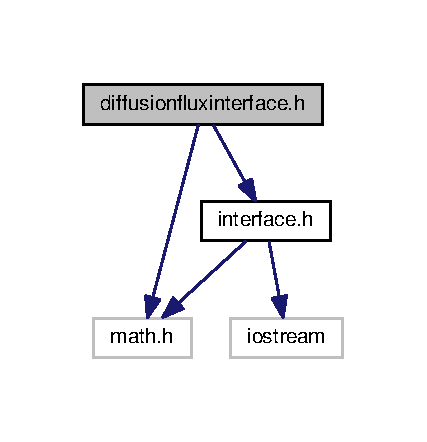
\includegraphics[width=205pt]{diffusionfluxinterface_8h__incl}
\end{center}
\end{figure}
This graph shows which files directly or indirectly include this file\+:
\nopagebreak
\begin{figure}[H]
\begin{center}
\leavevmode
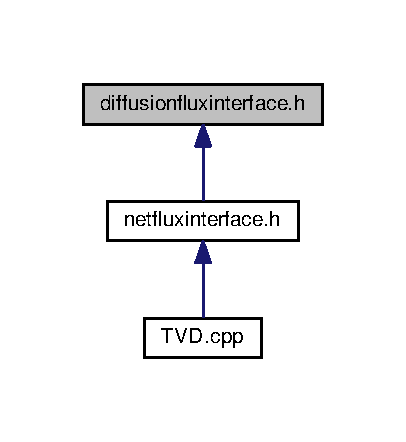
\includegraphics[width=199pt]{diffusionfluxinterface_8h__dep__incl}
\end{center}
\end{figure}
\subsection*{Classes}
\begin{DoxyCompactItemize}
\item 
class \hyperlink{classdiffusionfluxinterface}{diffusionfluxinterface}
\end{DoxyCompactItemize}


\subsection{Detailed Description}
This class calculates the numerical diffusion flux. 

\begin{DoxyAuthor}{Author}
Kuldeep Singh 
\end{DoxyAuthor}
\begin{DoxyDate}{Date}
2017 
\end{DoxyDate}
\begin{DoxyCopyright}{Copyright}
G\+NU Public License.
\end{DoxyCopyright}

\begin{DoxyParams}[1]{Parameters}
 & {\em Diffusion\+Flux\+Vector} & Numerical diffusion flux vector at the interface \\
\hline
\mbox{\tt in}  & {\em Conserved\+Variable} & Conserved variable vector (\mbox{[}Density , x-\/momentum, y-\/momentum, z-\/momentum, Energy\mbox{]}) \\
\hline
\mbox{\tt in}  & {\em Cell\+Vulume} & Pointer to the cell volume vector \\
\hline
\mbox{\tt in}  & {\em Left\+Minus} & Cell just previous to the left \\
\hline
\mbox{\tt in}  & {\em Right\+Plus} & Cell just Next to the right \\
\hline
\mbox{\tt in}  & {\em DeltaT} & Time step \\
\hline
\end{DoxyParams}
\begin{DoxyRefDesc}{Bug}
\item[\hyperlink{bug__bug000001}{Bug}]Needs to explain the code little bit more. \end{DoxyRefDesc}

\hypertarget{eulerflux_8h}{}\section{eulerflux.\+h File Reference}
\label{eulerflux_8h}\index{eulerflux.\+h@{eulerflux.\+h}}


This class calculates the euler flux vectors(\+Ee,\+Fe,\+Ge) at the interface.  


{\ttfamily \#include \char`\"{}math.\+h\char`\"{}}\\*
{\ttfamily \#include \char`\"{}iostream\char`\"{}}\\*
Include dependency graph for eulerflux.\+h\+:\nopagebreak
\begin{figure}[H]
\begin{center}
\leavevmode
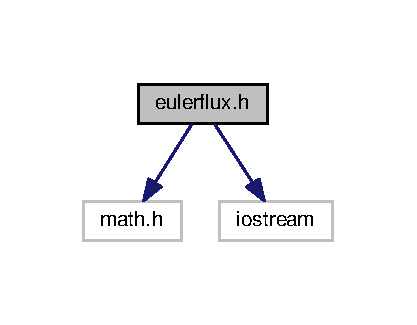
\includegraphics[width=200pt]{eulerflux_8h__incl}
\end{center}
\end{figure}
This graph shows which files directly or indirectly include this file\+:
\nopagebreak
\begin{figure}[H]
\begin{center}
\leavevmode
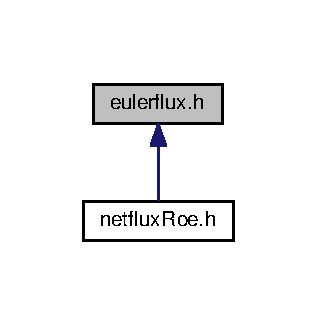
\includegraphics[width=172pt]{eulerflux_8h__dep__incl}
\end{center}
\end{figure}
\subsection*{Classes}
\begin{DoxyCompactItemize}
\item 
class \hyperlink{classeulerflux}{eulerflux}
\end{DoxyCompactItemize}
\subsection*{Macros}
\begin{DoxyCompactItemize}
\item 
\#define \hyperlink{eulerflux_8h_ab683b1fef77e9bd4205b818c943fec96}{Specific\+Heat\+Ratio}~1.\+4
\end{DoxyCompactItemize}


\subsection{Detailed Description}
This class calculates the euler flux vectors(\+Ee,\+Fe,\+Ge) at the interface. 

\begin{DoxyAuthor}{Author}
Kuldeep Singh 
\end{DoxyAuthor}
\begin{DoxyDate}{Date}
2017 
\end{DoxyDate}
\begin{DoxyRefDesc}{Bug}
\item[\hyperlink{bug__bug000004}{Bug}]Not all memory is freed when deleting an object of this class. \end{DoxyRefDesc}
\begin{DoxyCopyright}{Copyright}
G\+NU Public License. 
\end{DoxyCopyright}

\begin{DoxyParams}[1]{Parameters}
 & {\em Euler\+FluxX} & x direction euler flux vector (Ee) at interface \\
\hline
 & {\em Euler\+FluxY} & y direction euler flux vector (Fe) at interface \\
\hline
 & {\em Euler\+FluxZ} & z direction euler flux vector (Ge) at interface \\
\hline
\mbox{\tt in}  & {\em Conserved\+Variable} & Conserved variable vector (\mbox{[}Density , x-\/momentum, y-\/momentum, z-\/momentum, Energy\mbox{]}) \\
\hline
 & {\em Pressure} & Satic pressure (p) \\
\hline
\end{DoxyParams}


\subsection{Macro Definition Documentation}
\index{eulerflux.\+h@{eulerflux.\+h}!Specific\+Heat\+Ratio@{Specific\+Heat\+Ratio}}
\index{Specific\+Heat\+Ratio@{Specific\+Heat\+Ratio}!eulerflux.\+h@{eulerflux.\+h}}
\subsubsection[{\texorpdfstring{Specific\+Heat\+Ratio}{SpecificHeatRatio}}]{\setlength{\rightskip}{0pt plus 5cm}\#define Specific\+Heat\+Ratio~1.\+4}\hypertarget{eulerflux_8h_ab683b1fef77e9bd4205b818c943fec96}{}\label{eulerflux_8h_ab683b1fef77e9bd4205b818c943fec96}
This is gas constant (Gamma). For air at room temperature it is almost equal to 1.\+4. If you are using some other gas at some other temperature then change it 
\hypertarget{ghostcell_8h}{}\section{ghostcell.\+h File Reference}
\label{ghostcell_8h}\index{ghostcell.\+h@{ghostcell.\+h}}


This header file functions find the ghost cells area vectors and ghost cell volumes.  


{\ttfamily \#include $<$iostream$>$}\\*
{\ttfamily \#include \char`\"{}math.\+h\char`\"{}}\\*
{\ttfamily \#include $<$fstream$>$}\\*
{\ttfamily \#include $<$string$>$}\\*
{\ttfamily \#include $<$vector$>$}\\*
{\ttfamily \#include $<$cstdlib$>$}\\*
Include dependency graph for ghostcell.\+h\+:\nopagebreak
\begin{figure}[H]
\begin{center}
\leavevmode
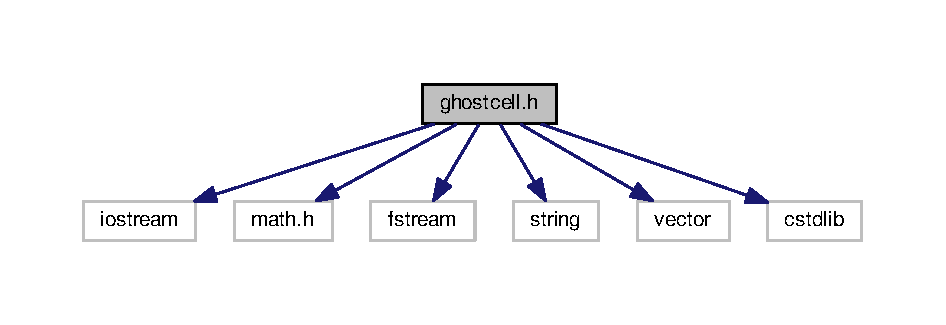
\includegraphics[width=350pt]{ghostcell_8h__incl}
\end{center}
\end{figure}
\subsection*{Functions}
\begin{DoxyCompactItemize}
\item 
void {\bfseries ghostcell} (vector$<$ vector$<$ vector$<$ vector$<$ double $>$ $>$ $>$ $>$ Coordinates, vector$<$ vector$<$ vector$<$ vector$<$ double $>$ $>$ $>$ $>$ i\+Face\+Area\+Vector, vector$<$ vector$<$ vector$<$ vector$<$ double $>$ $>$ $>$ $>$ j\+Face\+Area\+Vector, vector$<$ vector$<$ vector$<$ vector$<$ double $>$ $>$ $>$ $>$ k\+Face\+Area\+Vector, vector$<$ vector$<$ vector$<$ double $>$ $>$ $>$ Cell\+Volume, vector$<$ vector$<$ vector$<$ double $>$ $>$ $>$ \&i0\+Ghost\+Cell\+Volume, vector$<$ vector$<$ vector$<$ double $>$ $>$ $>$ \&j0\+Ghost\+Cell\+Volume, vector$<$ vector$<$ vector$<$ double $>$ $>$ $>$ \&k0\+Ghost\+Cell\+Volume, vector$<$ vector$<$ vector$<$ double $>$ $>$ $>$ \&i\+Ni\+Ghost\+Cell\+Volume, vector$<$ vector$<$ vector$<$ double $>$ $>$ $>$ \&j\+Nj\+Ghost\+Cell\+Volume, vector$<$ vector$<$ vector$<$ double $>$ $>$ $>$ \&k\+Nk\+Ghost\+Cell\+Volume, int Ni, int Nj, int Nk)\hypertarget{ghostcell_8h_ad6132b43473028e6ddf8fd37dda8d4fd}{}\label{ghostcell_8h_ad6132b43473028e6ddf8fd37dda8d4fd}

\end{DoxyCompactItemize}


\subsection{Detailed Description}
This header file functions find the ghost cells area vectors and ghost cell volumes. 

\begin{DoxyAuthor}{Author}
Kuldeep Singh 
\end{DoxyAuthor}
\begin{DoxyDate}{Date}
2017 
\end{DoxyDate}

\hypertarget{interface_8h}{}\section{interface.\+h File Reference}
\label{interface_8h}\index{interface.\+h@{interface.\+h}}


This class calculates the interface parameters using Reo scheme flux.  


{\ttfamily \#include \char`\"{}math.\+h\char`\"{}}\\*
{\ttfamily \#include \char`\"{}iostream\char`\"{}}\\*
Include dependency graph for interface.\+h\+:\nopagebreak
\begin{figure}[H]
\begin{center}
\leavevmode
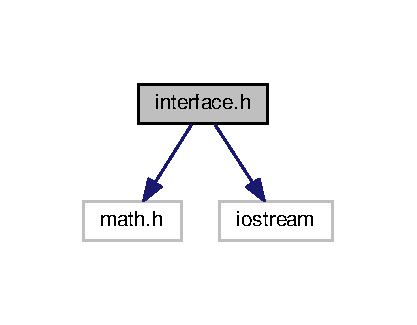
\includegraphics[width=200pt]{interface_8h__incl}
\end{center}
\end{figure}
This graph shows which files directly or indirectly include this file\+:
\nopagebreak
\begin{figure}[H]
\begin{center}
\leavevmode
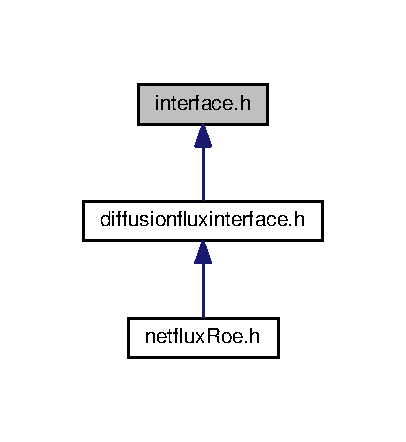
\includegraphics[width=199pt]{interface_8h__dep__incl}
\end{center}
\end{figure}
\subsection*{Classes}
\begin{DoxyCompactItemize}
\item 
class \hyperlink{classinterface}{interface}
\end{DoxyCompactItemize}
\subsection*{Macros}
\begin{DoxyCompactItemize}
\item 
\#define \hyperlink{interface_8h_ab683b1fef77e9bd4205b818c943fec96}{Specific\+Heat\+Ratio}~1.\+4
\end{DoxyCompactItemize}


\subsection{Detailed Description}
This class calculates the interface parameters using Reo scheme flux. 

\begin{DoxyAuthor}{Author}
Kuldeep Singh 
\end{DoxyAuthor}
\begin{DoxyDate}{Date}
2017 
\end{DoxyDate}
\begin{DoxyCopyright}{Copyright}
G\+NU Public License. 
\end{DoxyCopyright}

\begin{DoxyParams}[1]{Parameters}
 & {\em Density\+Interface} & Roe density at interface \\
\hline
 & {\em Velocity\+X\+Interface} & x velocity at interface \\
\hline
 & {\em Velocity\+Y\+Interface} & y velocity at interface \\
\hline
 & {\em Velocity\+Z\+Interface} & z velocity at interface \\
\hline
 & {\em Enthalpy\+Interface} & Enthalpy at interface \\
\hline
 & {\em Enthalpy\+Interface} & Enthalpy at interface \\
\hline
 & {\em Vector\+Jump\+Interface} & Change in the conserved parameters at the interface \\
\hline
 & {\em Eigen\+Value} & Eigenvalue of the Jacobian matrix \\
\hline
 & {\em Eigen\+Vector\+Matrix} & Eigenvector of the Jacobian matrix \\
\hline
 & {\em Eigen\+Vector\+Matrix\+Inverse} & Inverse of the Jacobian matrix \\
\hline
 & {\em Alpha\+Vector\+Interface\mbox{[}5\mbox{]}} & Eigen\+Vector\+Matrix\+Inverse\mbox{[}5\mbox{]}\mbox{[}5\mbox{]}$\ast$\+Vector\+Jump\+Interface \\
\hline
 & {\em Mu\+Vector\+Interface} & = delta t $\ast$ Eigen\+Value \\
\hline
 & {\em Z\+Vector\+Interface} & This is same as Mu\+Vector\+Interface \\
\hline
\mbox{\tt in}  & {\em Conserved\+Variables} & This is the pointer to the 4D vector where all the conserved variables of previous time step are stored. \\
\hline
\mbox{\tt in}  & {\em Face\+Area\+Vector\+Interface} & This is the pointer to the area vector the cell interface \\
\hline
 & {\em Cell\+Volume} & 3D vector which has the cell volume of all cells inside the domain \\
\hline
\end{DoxyParams}


\subsection{Macro Definition Documentation}
\index{interface.\+h@{interface.\+h}!Specific\+Heat\+Ratio@{Specific\+Heat\+Ratio}}
\index{Specific\+Heat\+Ratio@{Specific\+Heat\+Ratio}!interface.\+h@{interface.\+h}}
\subsubsection[{\texorpdfstring{Specific\+Heat\+Ratio}{SpecificHeatRatio}}]{\setlength{\rightskip}{0pt plus 5cm}\#define Specific\+Heat\+Ratio~1.\+4}\hypertarget{interface_8h_ab683b1fef77e9bd4205b818c943fec96}{}\label{interface_8h_ab683b1fef77e9bd4205b818c943fec96}
This is gas constant (Gamma). For air at room temperature it is almost equal to 1.\+4. If you are using some other gas at some other temperature then change it 
\hypertarget{local__time__step_8h}{}\section{local\+\_\+time\+\_\+step.\+h File Reference}
\label{local__time__step_8h}\index{local\+\_\+time\+\_\+step.\+h@{local\+\_\+time\+\_\+step.\+h}}


This header file conditions the function Time\+Step() which calculate the local time step for each cell at every iteration.  


{\ttfamily \#include $<$vector$>$}\\*
{\ttfamily \#include $<$math.\+h$>$}\\*
Include dependency graph for local\+\_\+time\+\_\+step.\+h\+:\nopagebreak
\begin{figure}[H]
\begin{center}
\leavevmode
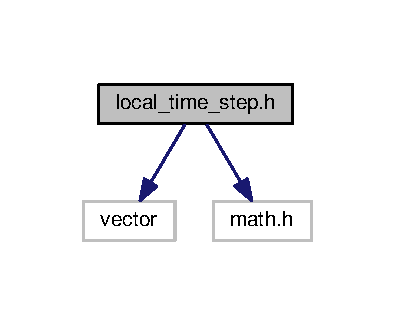
\includegraphics[width=190pt]{local__time__step_8h__incl}
\end{center}
\end{figure}
\subsection*{Functions}
\begin{DoxyCompactItemize}
\item 
double {\bfseries Time\+Step} (int i, int j, int k, vector$<$ vector$<$ vector$<$ double $>$ $>$ $>$ delta\+\_\+s, vector$<$ vector$<$ vector$<$ vector$<$ double $>$ $>$ $>$ $>$ Conserved\+Variables)\hypertarget{local__time__step_8h_a9a9d3b47de7cb00d45159818b69d0843}{}\label{local__time__step_8h_a9a9d3b47de7cb00d45159818b69d0843}

\end{DoxyCompactItemize}


\subsection{Detailed Description}
This header file conditions the function Time\+Step() which calculate the local time step for each cell at every iteration. 

\begin{DoxyAuthor}{Author}
Kuldeep Singh 
\end{DoxyAuthor}
\begin{DoxyDate}{Date}
2016 
\end{DoxyDate}
\begin{DoxySeeAlso}{See also}
\hyperlink{grid__ideal__nozzle_8h_a0195a06d59a6445d9ef8d27b775caeb0}{grid()} 
\end{DoxySeeAlso}
\begin{DoxyRefDesc}{Bug}
\item[\hyperlink{bug__bug000007}{Bug}]Currently not using this, because \hyperlink{grid__ideal__nozzle_8h_a0195a06d59a6445d9ef8d27b775caeb0}{grid()} is not calculating ds value. So recheck this function as well after fixing the \hyperlink{grid__ideal__nozzle_8h_a0195a06d59a6445d9ef8d27b775caeb0}{grid()} function. \end{DoxyRefDesc}

\begin{DoxyParams}[1]{Parameters}
\mbox{\tt in}  & {\em i,j,k} & Cell location for which Time\+Step is to be calculated \\
\hline
\mbox{\tt in}  & {\em delta\+\_\+s} & ds value of the cell for which Time\+Step is to be calculated \\
\hline
 & {\em \mbox{[}\+I\+N\mbox{]}} & Conserved\+Variables Conserved variables vector \\
\hline
 & {\em C\+FL} & Courant–\+Friedrichs–\+Lewy number \\
\hline
 & {\em Pressure} & Static Pressure \\
\hline
 & {\em Velocity\+Magnitude} & Magnitude of the velocity \\
\hline
 & {\em Velocity\+Sound} & Speed of sound \\
\hline
\mbox{\tt out}  & {\em Time\+Step} & Time step (dt) \\
\hline
\end{DoxyParams}
\begin{DoxyReturn}{Returns}
double 
\end{DoxyReturn}

\hypertarget{MainSolver_8cpp}{}\section{Main\+Solver.\+cpp File Reference}
\label{MainSolver_8cpp}\index{Main\+Solver.\+cpp@{Main\+Solver.\+cpp}}


This is the Main file which runs the simulation.  


{\ttfamily \#include \char`\"{}All\+Faces\+Flux\+A\+U\+S\+M.\+h\char`\"{}}\\*
{\ttfamily \#include \char`\"{}Boundary\+Netflux.\+h\char`\"{}}\\*
{\ttfamily \#include \char`\"{}Deltat.\+h\char`\"{}}\\*
{\ttfamily \#include \char`\"{}Residual.\+h\char`\"{}}\\*
{\ttfamily \#include \char`\"{}Initial\+Condition.\+h\char`\"{}}\\*
{\ttfamily \#include \char`\"{}Grid.\+h\char`\"{}}\\*
{\ttfamily \#include \char`\"{}Ghostcell.\+h\char`\"{}}\\*
{\ttfamily \#include \char`\"{}Array\+Tester.\+h\char`\"{}}\\*
{\ttfamily \#include \char`\"{}Conserved\+Quantities\+Writer.\+h\char`\"{}}\\*
{\ttfamily \#include \char`\"{}Colortext.\+h\char`\"{}}\\*
Include dependency graph for Main\+Solver.\+cpp\+:\nopagebreak
\begin{figure}[H]
\begin{center}
\leavevmode
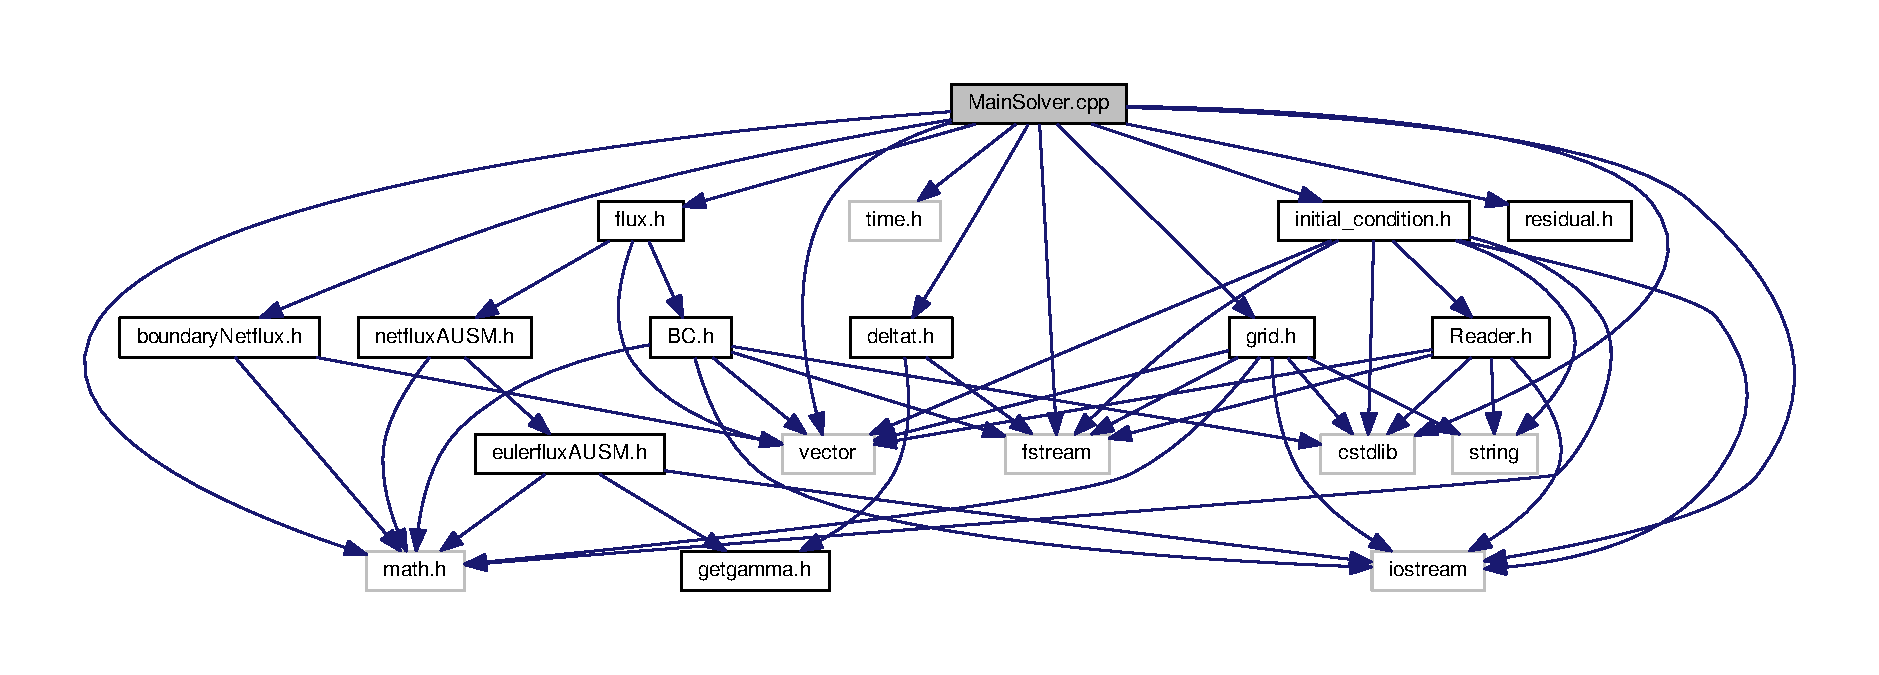
\includegraphics[width=350pt]{MainSolver_8cpp__incl}
\end{center}
\end{figure}
\subsection*{Functions}
\begin{DoxyCompactItemize}
\item 
int \hyperlink{MainSolver_8cpp_ae66f6b31b5ad750f1fe042a706a4e3d4}{main} ()
\end{DoxyCompactItemize}


\subsection{Detailed Description}
This is the Main file which runs the simulation. 

\begin{DoxyAuthor}{Author}
Kuldeep Singh 
\end{DoxyAuthor}
\begin{DoxyDate}{Date}
May, 2017 
\end{DoxyDate}


\subsection{Function Documentation}
\index{Main\+Solver.\+cpp@{Main\+Solver.\+cpp}!main@{main}}
\index{main@{main}!Main\+Solver.\+cpp@{Main\+Solver.\+cpp}}
\subsubsection[{\texorpdfstring{main()}{main()}}]{\setlength{\rightskip}{0pt plus 5cm}int main (
\begin{DoxyParamCaption}
{}
\end{DoxyParamCaption}
)}\hypertarget{MainSolver_8cpp_ae66f6b31b5ad750f1fe042a706a4e3d4}{}\label{MainSolver_8cpp_ae66f6b31b5ad750f1fe042a706a4e3d4}

\begin{DoxyParams}{Parameters}
{\em Start\+Time} & Simulation starting time\\
\hline
{\em End\+Time} & Simulation ending time\\
\hline
{\em Total\+Iteration} & Total iterations\\
\hline
{\em Scheme} & \char`\"{}\+A\+U\+S\+M\char`\"{} or \char`\"{}\+Roe\char`\"{}\\
\hline
{\em Time\+Steping} & Whether to use local \char`\"{}delta t\char`\"{} or global \char`\"{}delta t\char`\"{}\\
\hline
{\em Geometry\+Option} & Using this option grids (area vector and the cell volumes) will be defined appropriately\\
\hline
{\em gamma} & Option, whether constant Specific heat ratio is constant or variable\\
\hline
{\em C\+FL} & \\
\hline
{\em Specific\+Heat\+Ratio} & Specific heat ratio in case of constant gamma\\
\hline
{\em deltat} & Time step\\
\hline
\end{DoxyParams}
Reading the input file

Reading the input file over


\begin{DoxyParams}{Parameters}
{\em Ni} & Number of live cells in in \char`\"{}i\char`\"{} direction.\\
\hline
{\em Nj} & Number of live cells in in \char`\"{}j\char`\"{} direction.\\
\hline
{\em Nk} & Number of live cells in in \char`\"{}k\char`\"{} direction.\\
\hline
\end{DoxyParams}
\begin{DoxyWarning}{Warning}
Final value of the Ni,Nj,Nk has been decided inside the \hyperlink{Grid_8h_a431e327cd64293b7c55a97f1a91f70de}{grid()} function. So, do not use these parameters until the grid function is called
\end{DoxyWarning}

\begin{DoxyParams}{Parameters}
{\em Coordinates} & This is a 4D vector which has the coordinated of all vertices\textquotesingle{}s\\
\hline
{\em i\+Face\+Area\+Vector} & This is a 4D vector which has the area vector of all faces which are in \char`\"{}i\char`\"{} direction.\\
\hline
{\em j\+Face\+Area\+Vector} & This is a 4D vector which has the area vector of all faces which are in \char`\"{}j\char`\"{} direction.\\
\hline
{\em k\+Face\+Area\+Vector} & This is a 4D vector which has the area vector of all faces which are in \char`\"{}k\char`\"{} direction.\\
\hline
{\em Cell\+Volume} & Input pointer to cell volumes\\
\hline
{\em delta\+\_\+s} & Minimum distance\\
\hline
\end{DoxyParams}
After calling grid function all the live cell quantities will be decided

Testing the array declared using grid function


\begin{DoxyParams}{Parameters}
{\em i0\+Ghost\+Cell\+Volume} & Ghost cell volume array at i = 0\\
\hline
{\em j0\+Ghost\+Cell\+Volume} & Ghost cell volume array at j = 0\\
\hline
{\em k0\+Ghost\+Cell\+Volume} & Ghost cell volume array at k = 0\\
\hline
{\em i\+Ni\+Ghost\+Cell\+Volume} & Ghost cell volume array at i = Ni\\
\hline
{\em j\+Nj\+Ghost\+Cell\+Volume} & Ghost cell volume array at j = Nj\\
\hline
{\em k\+Nk\+Ghost\+Cell\+Volume} & Ghost cell volume array at k = Nk\\
\hline
{\em Conserved\+Variables} & This is the pointer to the 4D vector where all the conserved variables (\mbox{[}Density , x-\/momentum, y-\/momentum, z-\/momentum, Energy\mbox{]}) of previous time step are stored.\\
\hline
{\em Conserved\+Variables\+New} & This is the pointer to the 4D vector where all the conserved variables (\mbox{[}Density , x-\/momentum, y-\/momentum, z-\/momentum, Energy\mbox{]}) of current/new time step are stored.\\
\hline
\end{DoxyParams}
Initializing the domain


\begin{DoxyParams}{Parameters}
{\em i\+Faces\+Flux} & This is a 4D vector which has the fluxes of all faces which are in \char`\"{}i\char`\"{} direction.\\
\hline
{\em j\+Faces\+Flux} & This is a 4D vector which has the fluxes of all faces which are in \char`\"{}j\char`\"{} direction.\\
\hline
{\em k\+Faces\+Flux} & This is a 4D vector which has the fluxes of all faces which are in \char`\"{}k\char`\"{} direction.\\
\hline
\end{DoxyParams}
Opening the \char`\"{}\+Residual.\+csv\char`\"{} file to store the all the residuals

Iterations starts here

calculating the global time step after every time iteration

Calculating the local \char`\"{}delta t\char`\"{} here


\begin{DoxyParams}{Parameters}
{\em Net\+Flux} & Normal component of the flux across the interface\\
\hline
\end{DoxyParams}
Updating the previous time step conserved quantities

before going to the new time step updating the old conserved variables by new ones

Writing the Conserved quantities in the output file

Simulation ends here 
%--- End generated contents ---

% Index
\backmatter
\newpage
\phantomsection
\clearemptydoublepage
\addcontentsline{toc}{chapter}{Index}
\printindex

\end{document}
